\documentclass{standalone}
\usepackage{tikz}
\begin{document}

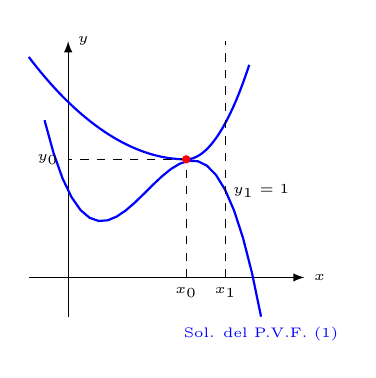
\begin{tikzpicture}[>=latex]
	\draw [->] (-0.5,0) -- (3,0) node [right] {\tiny \(x\)};
	\draw [->] (0,-0.5) -- (0,3) node [right] {\tiny \(y\)};
	\draw [blue, thick] (-0.5,2.8) parabola bend (1.5,1.5) (2.3,2.7);
	\draw [shift={(1,1.1)},thick ,blue, domain=-1.3:1.45] plot(\x , {-pow(\x,3) +\x}) node [below] {\tiny Sol. del P.V.F. (1)};
	\draw [dashed] (1.5,0) node [below] {\tiny \(x_0\)} -- (1.5,1.5) -- (0,1.5) node [left] {\tiny \(y_0\)};
	\draw [dashed] (2,0) node [below] {\tiny \(x_1\)} --++ (0,3);
	\node at (2.45,1.1) {\tiny \(y_1=1\)};
	\fill [red] (1.5,1.5) circle (1.5pt);
\end{tikzpicture}

\end{document}
